\section{Aprendizado de máquina}

Aprendizado pode ser definido como qualquer mudança em um sistema que
otimize o seu desempenho na segunda vez que ele repetir a mesma tarefa,
ou outra tarefa da mesma população~\cite{custodio2010aprendizadomaquina}.

O aprendizado de máquina utiliza um princípio de inferência denominado
indução, onde através de um conjunto particular de exemplos é possível
obter conclusões genéricas~\cite{bruno2010aprendizadomaquina}. De um modo
abstrato o aprendizado de máquina funciona como uma caixa preta, onde
independente de como é implementado, o algoritmo deve ser capaz de receber
várias entradas com suas respectivas saídas, como informações de treinamento,
essa é a parte aonde ocorre o aprendizado, após isso o algoritmo deve
ser capaz de apresentar um resultado para cada novo dado de entrada no
algoritmo, onde quanto melhor for o treinamento, melhor os resultados
dos novos dados de entrada.

Como exemplo, o aprendizado de máquina pode ser usado para identificar
um número em uma imagem. Supondo que uma imagem seja uma matriz de pixels
28x28 e que os pixels estão em escala de cinza, ou seja, vão de 0 a 255, e
que essa imagem se trata de um número, o algoritmo deve receber várias
entradas como treinamento, contendo a imagem e o número que corresponde a
essa imagem. Após o treinamento o programa deve ser capaz de
receber uma imagem 28x28 e identificar qual número está na imagem.

\subsection{Aprendizado supervisionado}

Uma das principais técnicas de aprendizado de máquina é o aprendizado
supervisionado, onde é fornecido um treinamento com o conhecimento do
ambiente, o treinamento é composto por um conjunto de exemplos com entradas
e uma saída esperada~\cite{bruno2010aprendizadomaquina}.

O objetivo do aprendizado supervisionado é induzir conceitos a partir de
exemplos que estão pré-classificados, em outras palavras, exemplos que
possuem um rótulo associado a uma classe conhecida~\cite{bruno2010aprendizadomaquina}.
Utilizado quando se tem tanto as perguntas quanto as respostas, o aprendizado
supervisionado é utilizado para se obter uma classificação e funções de aproximação.

Utilizando do exemplo do algoritmo que identifica um número em uma imagem,
na utilização do aprendizado supervisionado para cada entrada no treinamento
há um rótulo, que é um número de 0 a 9, que identifica qual número está na
imagem, e uma sequencia de 784 pixels que representam a matriz 28x28 da imagem.
A figura~\ref{fig:tabela_ml_treinamento} mostra um exemplo das entradas de
treinamento.

\begin{figure}[h]
  \centering
  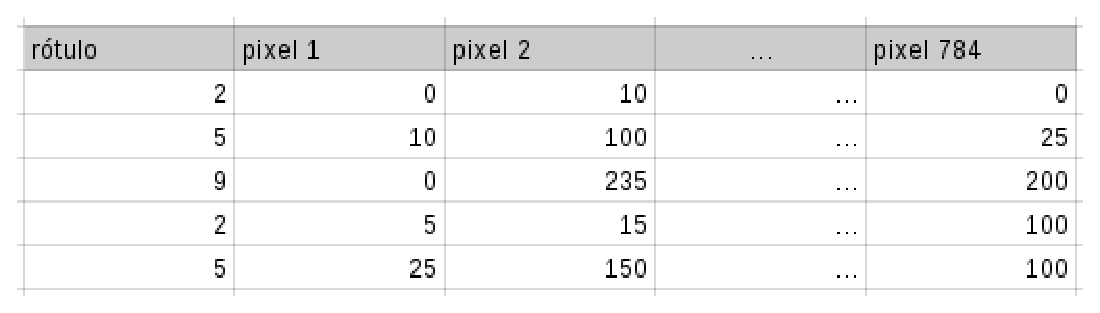
\includegraphics[width=0.9\textwidth]{figuras/tabela_ml_treinamento.eps}
  \caption{Entradas de treinamento para o aprendizado de máquina}
  \label{fig:tabela_ml_treinamento}
\end{figure}

Após ser realizada a etapa de treinamento, ao receber uma sequencia de 784
pixels, o algoritmo deve responder qual o rótulo, que é o número de 0 a 9,
correspondente a sequencia de 784 pixels. A figura~\ref{fig:tabela_ml_entrada}
mostra um exemplo de uma entrada para o algoritmo, a diferença dessa entrada
para uma entrada de treinamento é que essa não possui o rótulo, pois o rótulo
será o resultado da execução do algoritmo.

\begin{figure}[h]
  \centering
  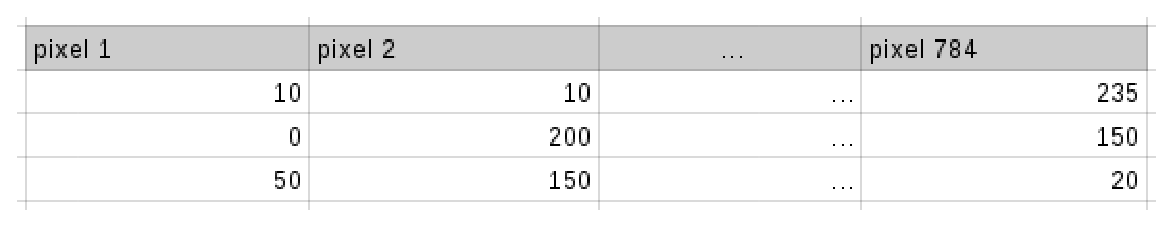
\includegraphics[width=0.9\textwidth]{figuras/tabela_ml_entrada.eps}
  \caption{Entradas de dados para o algoritmo determinar o rótulo}
  \label{fig:tabela_ml_entrada}
\end{figure}

\subsubsection{Bayes Ingênuo}

Um algoritmo supervisionado, e bastante utilizado no aprendizado de máquina,
o bayes ingênuo, também conhecido como naive bayes, é denominado ingênuo devido
ao fato de que o algoritmo assume que os atributos são condicionalmente
independentes, ou seja, considera-se que as entradas são independentes entre
si, porém, mesmo partindo dessa ingenuidade os resultados não comprometem a
qualidade~\cite{bruno2010aprendizadomaquina}. Mesmo com essa independencia dos
atributos, o bayes ingênuo é um método bastante efetivo e frequentemente oferece
uma precisão comparável aos outros métodos (comparável à métodos pertencentes ao
estado da arte), e estudos também mostram que o bayes ingênuo pode aprender a
função de classificação ótima~\cite{santos2010naivebayes}.

No caso do reconhecimento de um número em uma imagem 28x28, o vetor de pixels
que forma a imagem, ilustrado na figura~\ref{fig:tabela_ml_treinamento}, será
reescrito de forma que só irá possuir os valor 0 ou 255, por exemplo, todos os
pixels a baixo de 50 serão considerados como 0, e todos os pixels com valor igual
ou maior a 50 serão considerados como como 255, ou seja, a imagem ficará em preto
e branco, como mostra a figura~\ref{fig:tabela_ml_treinamento_convertida}.

\begin{figure}[h]
  \centering
  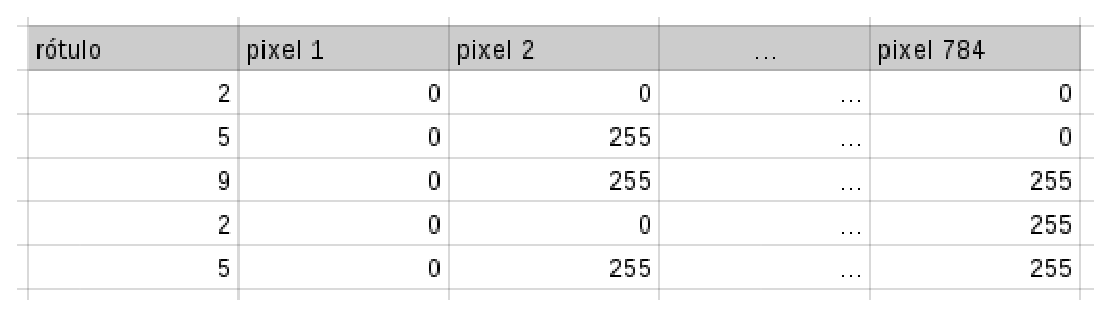
\includegraphics[width=0.9\textwidth]{figuras/tabela_ml_treinamento_convertida.eps}
  \caption{Entradas modificadas de treinamento para o aprendizado de máquina}
  \label{fig:tabela_ml_treinamento_convertida}
\end{figure}

Utilizando agora o vetor de pixels da figura~\ref{fig:tabela_ml_treinamento_convertida}
é necessário realizar o treinamento do algortitmo, onde se deve armazenar as informações
dos rótulo referente a cada pixel no vetor de pixels, onde para cada rótulo deve ser
armazenado quantos pixels 0 e quantos pixels 255 o rótulo possui para cada pixe, por
exemplo, o rótulo dois possui dois pixels zero e nenhum pixel 255 na primeira posição do
vetor de pixel, e possui um pixel 0 e um pixel 255 na ultima posição do vetor. Realizando
esse processo para todos os rótulos em todos os pixels do vetor que forma a imagem, a
contagem de quantos pixels diferentes cada rótulo possui é ilustrada na
figura~\ref{fig:tabela_ml_treinamento_convertida}.

\begin{figure}[h]
  \centering
  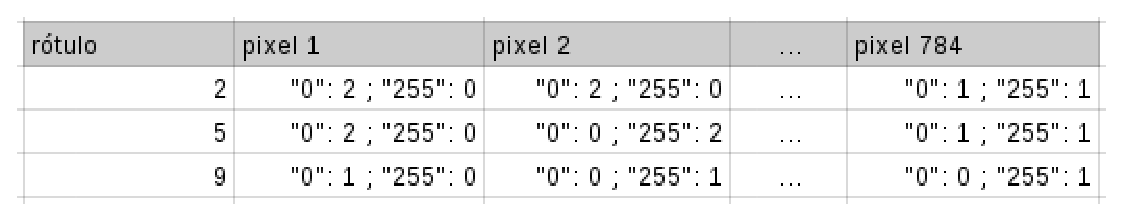
\includegraphics[width=0.9\textwidth]{figuras/rotulos_e_pixels.eps}
  \caption{Rótulos e sua quantidade de pixels para cada pixel do vetor que forma a imagem}
  \label{fig:rotulos_e_pixels}
\end{figure}

Após a realização do treinamento, resultando em dados como mostra a
figura~\ref{fig:tabela_ml_treinamento_convertida}, o algoritmo agora está pronto para
receber dados de entrada, um vetor contendo os 784 pixels que formam a imagem, e então
retornar qual o número que está na imagem. Para a entrada ilustrada na
figura~\ref{fig:bayes_dado_entrada}, o algoritmo convert para o formato onde os
pixels são classificados em 0 ou 255, como mostra a figura~\ref{fig:bayes_dado_entrada_convertida},

\begin{figure}[h]
  \centering
  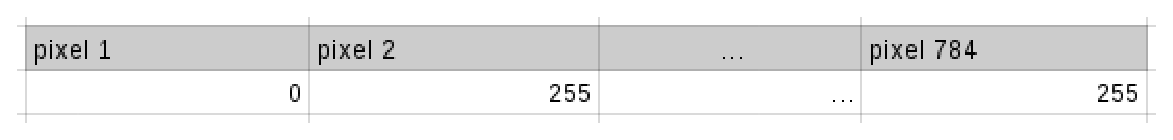
\includegraphics[width=0.9\textwidth]{figuras/bayes_dado_entrada_convertida.eps}
  \caption{Rótulos e sua quantidade de pixels para cada pixel do vetor que forma a imagem}
  \label{fig:bayes_dado_entrada_convertida}
\end{figure}

\begin{figure}[h]
  \centering
  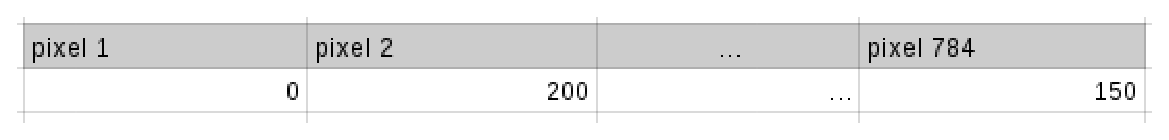
\includegraphics[width=0.9\textwidth]{figuras/bayes_dado_entrada.eps}
  \caption{Rótulos e sua quantidade de pixels para cada pixel do vetor que forma a imagem}
  \label{fig:bayes_dado_entrada}
\end{figure}
